\begin{figure}[t!]
\begin{flushright}
    % \raisebox{8.5\height}{\textbf{a}}
    \raisebox{.35\height}{\rotatebox{90}{\textbf{U-Maze}}}\hspace*{\fill}
    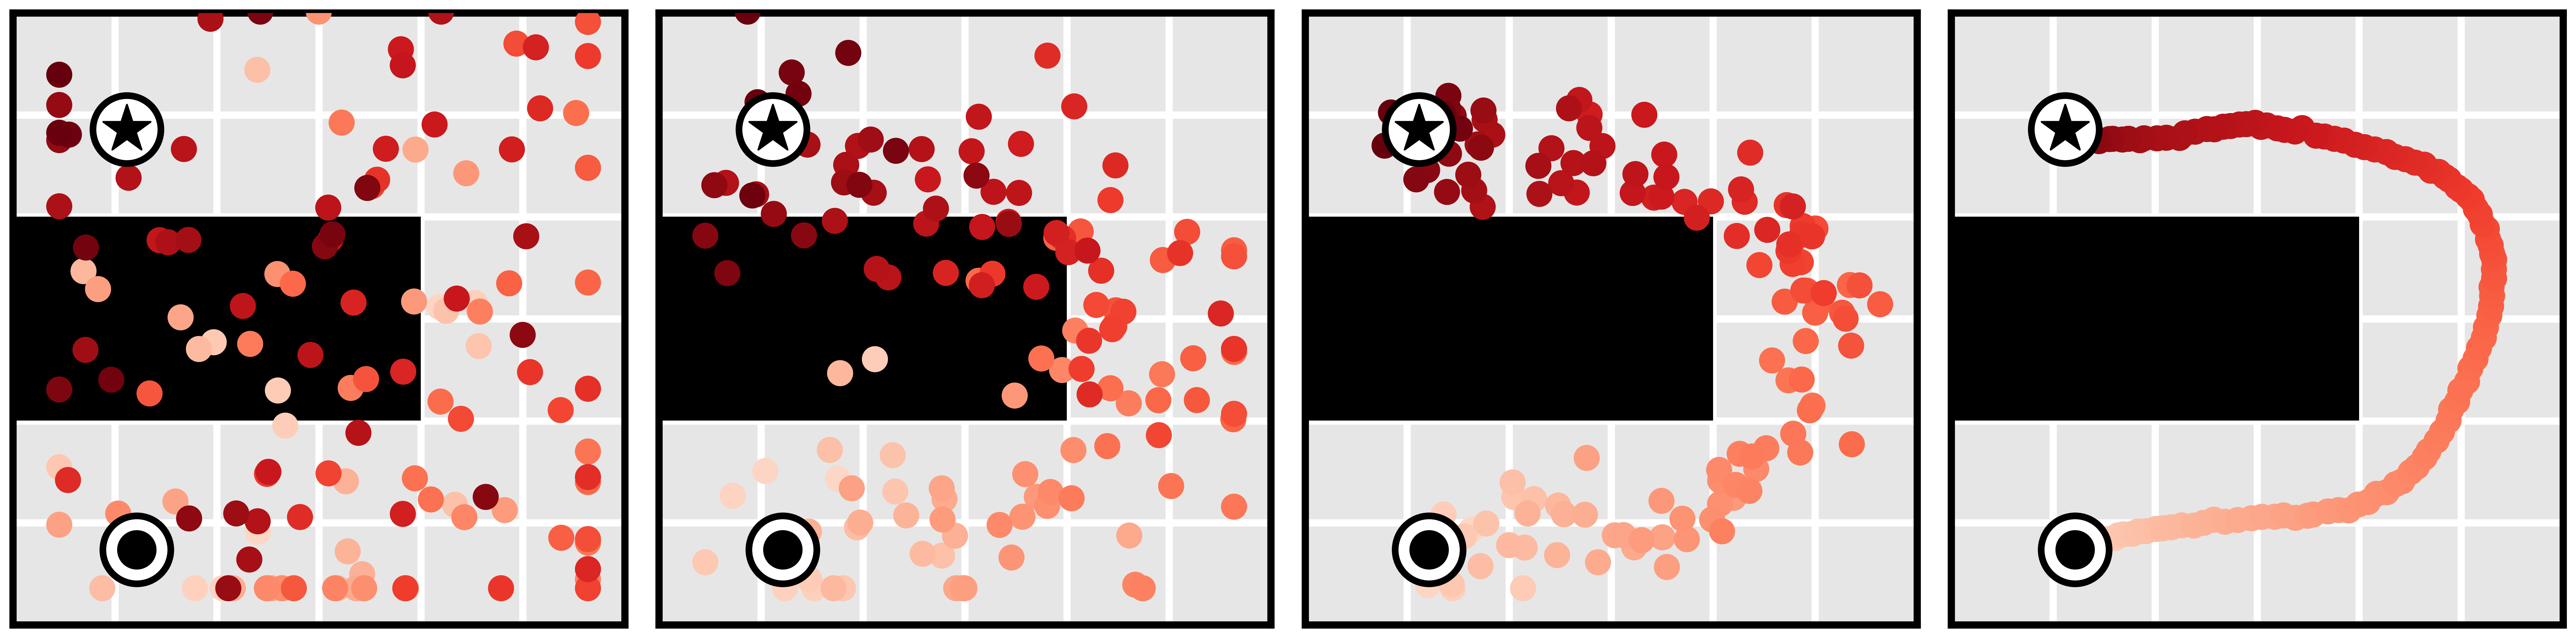
\includegraphics[width=0.95\columnwidth]{images/maze2d/maze2d-umaze-v1.png} \\
    %%
    % \raisebox{6.5\height}{\textbf{b}}
    \raisebox{.3\height}{\rotatebox{90}{\textbf{Medium}}}\hspace*{\fill}
    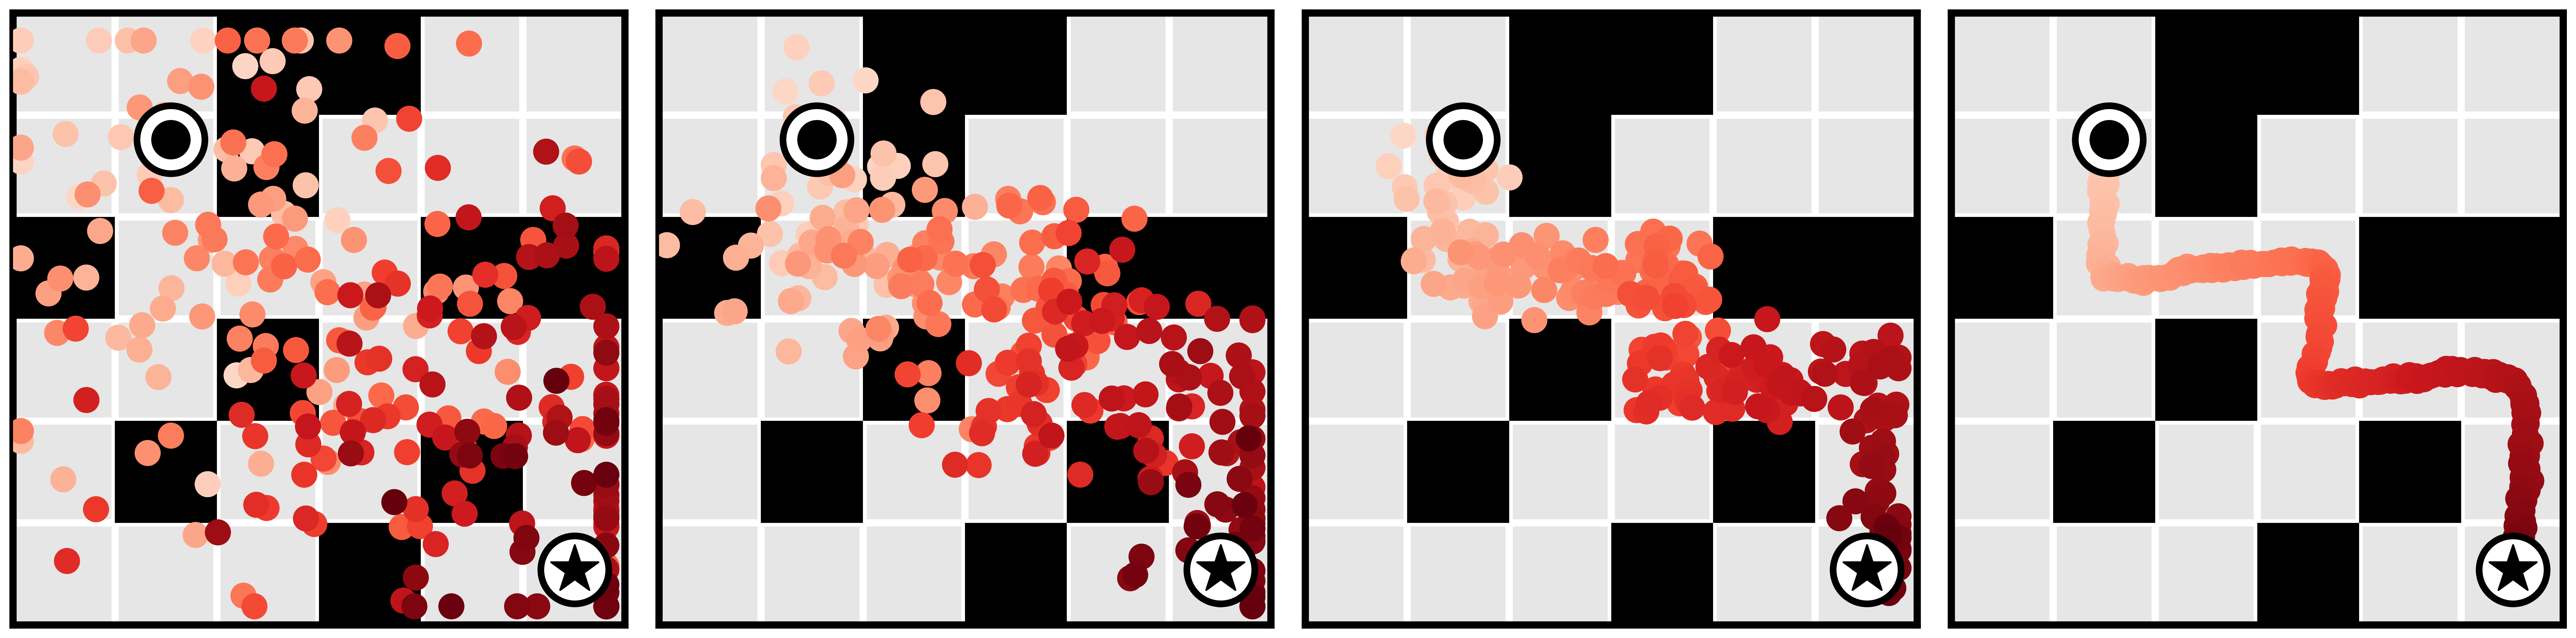
\includegraphics[width=0.95\columnwidth]{images/maze2d/maze2d-medium-v1.png} \\
    %%
    % \raisebox{8.5\height}{\textbf{c}}
    \raisebox{.6\height}{\rotatebox{90}{\textbf{Large}}}\hspace*{\fill}
    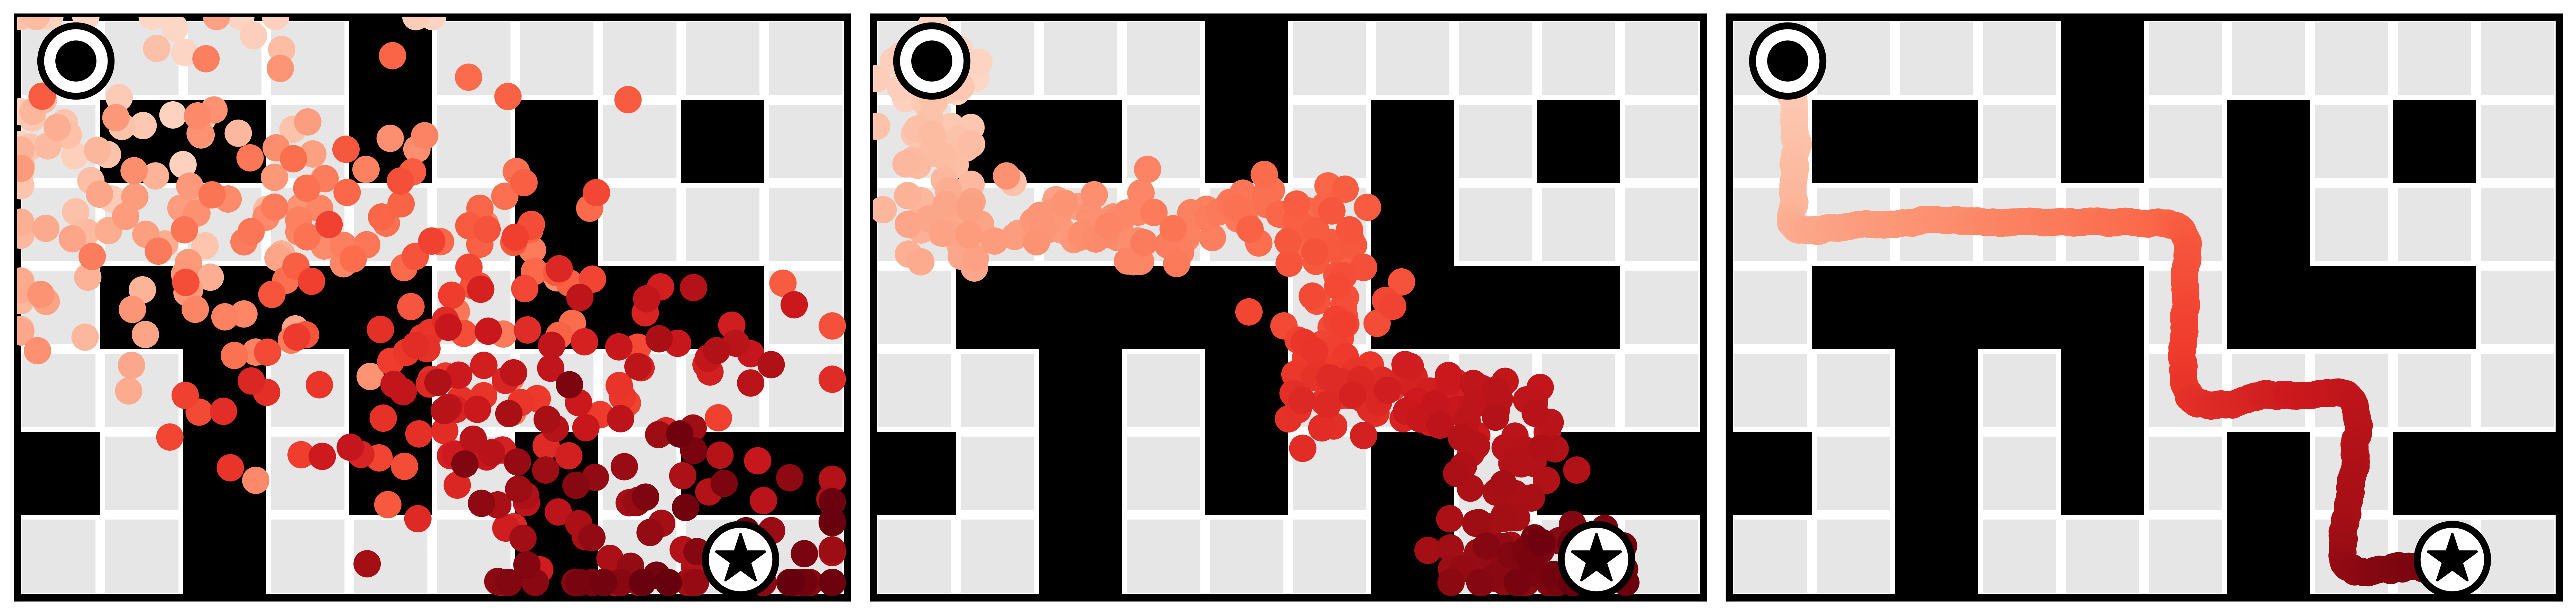
\includegraphics[width=0.95\columnwidth,trim={.03cm 0 .03cm 0},clip]{images/maze2d/maze2d-large-v1.png} \\
\end{flushright}
\begin{centering}
    \raisebox{.3\height}{denoising}~~
    \tikz \draw [-{Computer Modern Rightarrow[length=2mm, width=3mm]}, line width=.3mm] (0,0) -- (3,0); \\
    % \tikz \draw [-{Straight Barb[length=2mm, width=3mm]}, line width=.3mm] (0,0) -- (3,0); \\
\end{centering}
% \vspace{-4pt}
\caption{
    % \small
    \textbf{(Planning as inpainting)}
    Plans are generated in the Maze2D environment by sampling trajectories consistent with a specified start 
    \protect{\raisebox{-.05cm}{
\includegraphics[height=.35cm]{images/maze2d/mark_start_crop.png}}}
    and goal
    \protect{\raisebox{-.05cm}{
\includegraphics[height=.35cm]{images/maze2d/mark_goal_crop.png}}}
    condition.
    The remaining states are ``inpainted'' by the denoising process.
}
% \vspace{-.65cm}
\label{fig:maze2d}
\end{figure}